% Project report - compile with pdflatex (twice, for references),
% or upload the whole report/ folder to Overleaf.
% Each section lives in its own file in sections/, so the three of us can
% write in parallel without merge conflicts.
\documentclass[11pt,a4paper]{article}

\usepackage[utf8]{inputenc}
\usepackage[T1]{fontenc}
\usepackage{lmodern}
\usepackage[margin=2cm]{geometry}
\usepackage{graphicx}
\usepackage{booktabs}
\usepackage{amsmath}
\usepackage{xcolor}
\usepackage[font=small]{caption}
\usepackage{enumitem}
\setlist{itemsep=1pt,topsep=3pt}
\usepackage{float}
\usepackage[hidelinks]{hyperref}

\graphicspath{{figures/}}

% Placeholders for results that come from the full runs: remove them all
% before submitting (search for "TODO").
\newcommand{\todo}[1]{\textcolor{red}{\textbf{[TODO: #1]}}}
\newcommand{\todofigure}[1]{%
  \fbox{\parbox{0.9\textwidth}{\centering\vspace{1.2cm}%
  \textcolor{red}{\textbf{TODO figure:} #1}\vspace{1.2cm}}}}

% Notation used throughout the text.
\newcommand{\pos}{\mbox{$>$50K}}
\newcommand{\negc}{\mbox{$\leq$50K}}
\newcommand{\code}[1]{\texttt{#1}}

\title{Predicting an income above 50K from census data:\\
an end-to-end supervised learning proof of concept}
\author{Eduardo Pepe \and Louis Pimont-Nishimura \and Jules Faucher}
\date{MSA-DATB09-04 Supervised Learning \& Model Engineering, Albert School\\
Instructor: Ilana Sebag\\[4pt] October 2026}

\begin{document}

\maketitle

\noindent\textbf{Dataset:} Adult / Census Income, OpenML (\code{name="adult"}, \code{version=2}).\\
\textbf{Code:} \url{https://github.com/epepe-10/supervised-learning-project}

\section{Introduction}
\label{sec:intro}

\todo{problem, dataset, protocol in one paragraph, scope (fairness removed), structure of the report}

\section{Exploratory analysis and problem framing}
\label{sec:eda}

\subsection{Data integrity}

The raw table has 48{,}842 rows and 14 features: 6 integers and 8 categories. We
checked the meaning of each column, not only its storage type, which led to
three cleaning decisions.
\begin{itemize}
  \item \textbf{Missing values} appear only in three categorical columns:
  \code{workclass} (5.7\%), \code{occupation} (5.8\%) and \code{native-country}
  (1.8\%). They are imputed inside the Pipeline (Section~\ref{sec:features}),
  never before the split.
  \item \textbf{52 exact duplicate rows} (0.1\%) are dropped before the split,
  so the same record cannot end up both in a training fold and in the matching
  validation fold, or both in the development and the test set.
  \item \textbf{Two columns are not given to the model.} \code{education} and
  \code{education-num} have 16 values each and map one-to-one: each label has
  exactly one number and each number exactly one label. We keep
  \code{education-num}, which also carries the order of the levels.
  \code{fnlwgt} is a sampling weight of the census survey: it describes how the
  survey was designed, not the person whose income we predict.
\end{itemize}

\subsection{Validation protocol}

Each row is one person and there is no time dimension, so a random split is
appropriate. We split the cleaned data (48{,}790 rows) once, stratified on the
target, into a development set of 39{,}032 rows and a test set of 9{,}758 rows.
Both contain 23.9\% of \pos. Inside the development set, every comparison uses
the same 5-fold \code{StratifiedKFold} (shuffled, seed 42), so all models are
scored on exactly the same folds. Everything that relates the features to the
target, including the analysis below, was done on the development set only:
looking at the test set would already be a modelling decision.

\subsection{Target and choice of metrics}

The development set has 29{,}687 people at \negc{} and 9{,}345 at \pos. A model
that always predicts \negc{} is already 76.1\% accurate, so accuracy alone says
little. We report the same metrics for every model: ROC-AUC and Average
Precision (AP, the area under the precision-recall curve), which judge how well
people are ranked, without a threshold; log-loss, which judges the
probabilities; and precision, recall, F1 and the confusion matrix, which judge
the final decisions at a given threshold. AP is our selection metric: it focuses
on how well the minority class is retrieved, and its reference value is the
prevalence (0.239), against 0.5 for ROC-AUC.

\subsection{Main findings}

Table~\ref{tab:eda-means} compares the numerical features between the two
classes (the full distributions are in Figure~\ref{fig:eda-numeric}, in the
appendix). People earning \pos{} are older, more educated and work more hours.
\code{capital-gain} and \code{capital-loss} are zero for 91.8\% and 95.2\% of
people, with a long tail of large values. The share of \pos{} rises with age,
peaks around 50 and then falls (Figure~\ref{fig:eda-age}): a curve that a
linear model cannot draw with \code{age} alone. Among the categorical features
(Figure~\ref{fig:eda-categorical}), the household variables separate the
classes most: the share of \pos{} ranges from 5\% to 45\% across
\code{marital-status} values and from 2\% to 47\% across \code{relationship}
values. It is 30\% for men and 11\% for women.

\begin{table}[H]
\centering
\caption{Mean of each numerical feature by class (development set).}
\label{tab:eda-means}
\begin{tabular}{lrrrrr}
\toprule
Class & age & education-num & capital-gain & capital-loss & hours-per-week \\
\midrule
\negc & 36.9 & 9.6 & 144 & 54 & 38.8 \\
\pos  & 44.3 & 11.6 & 4{,}096 & 200 & 45.5 \\
\bottomrule
\end{tabular}
\end{table}

\begin{figure}[H]
\centering
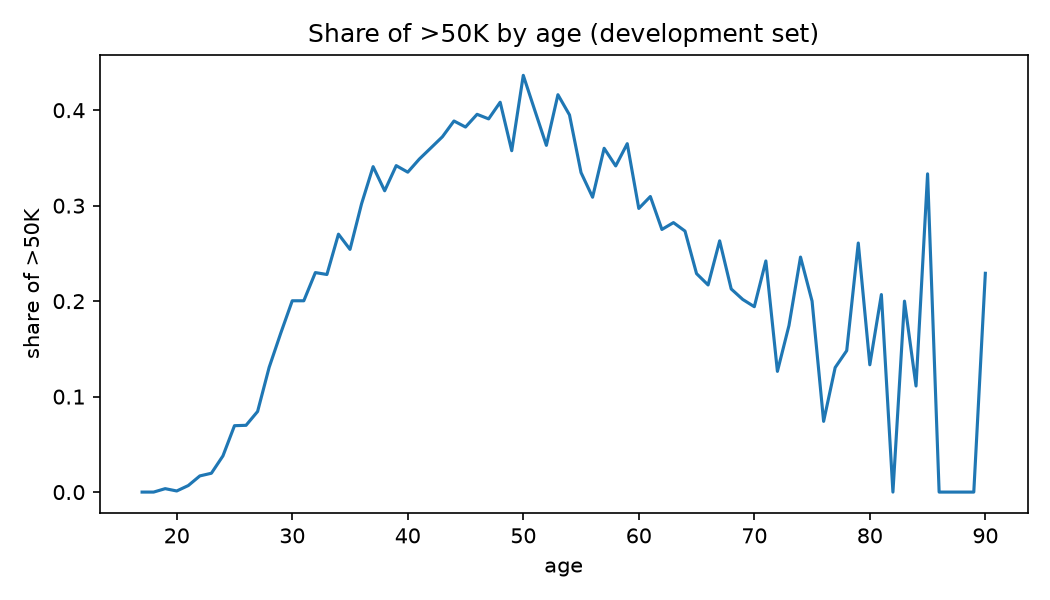
\includegraphics[width=0.55\textwidth]{eda_rate_by_age.png}
\caption{Share of \pos{} by age (development set): an inverted U, which
motivates the \code{age\_squared} feature.}
\label{fig:eda-age}
\end{figure}

\subsection{Leakage audit}

For each feature, we asked whether its value would really be known at the
moment the prediction is made (Table~\ref{tab:leakage}). Personal
characteristics, education, job and household are known in advance.
\code{capital-gain} and \code{capital-loss} are a medium risk: they are declared
for the same tax year as the income, so in production they might only become
available together with the income itself. We keep them, because the census
collects them at the same time as the other answers, but this must be checked
before any real deployment.

\begin{table}[H]
\centering
\caption{Leakage audit: could we know this value when the prediction is made?}
\label{tab:leakage}
\small
\begin{tabular}{p{4.6cm}p{2.4cm}p{2.2cm}p{5.2cm}}
\toprule
Features & Known at prediction time & Risk & Why \\
\midrule
age, sex, race, native-country & Yes & Low & Fixed personal characteristics \\
education-num & Yes & Low & Obtained before the income is earned \\
workclass, occupation, hours-per-week & Yes & Low & Describe the current job \\
marital-status, relationship & Yes & Low & Household situation \\
capital-gain, capital-loss & Same tax year & Medium & Declared with the income \\
fnlwgt & Yes & Not a person feature & Survey weight, dropped \\
\bottomrule
\end{tabular}
\end{table}

\subsection{Open questions}

Two assumptions remain open after the analysis. First, missing \code{workclass}
and \code{occupation} values may not be random: they could describe people who
do not work (we test this in Section~\ref{sec:discussion}). Second, the data
dates from 1994: income levels have changed since, so the \$50K threshold does
not mean the same today, and the model should not be used on recent data
without retraining.

\section{Feature engineering and preprocessing}
\label{sec:features}

\subsection{Three engineered features}

A logistic regression is linear in the log-odds: it cannot draw a curve, a
threshold or an interaction on its own. We gave it these shapes explicitly,
with one feature of each kind, each motivated by the analysis above.
\begin{itemize}
  \item \code{age\_squared} $= \text{age}^2$ (square term). With \code{age} and
  \code{age\_squared}, the model can draw the inverted U of
  Figure~\ref{fig:eda-age} instead of a straight line.
  \item \code{education\_x\_hours} $= \text{education-num} \times
  \text{hours-per-week}$ (interaction). The value of an extra hour of work is
  likely to depend on the level of education.
  \item \code{has\_capital} $= \mathbf{1}[\text{capital-gain} > 0 \text{ or }
  \text{capital-loss} > 0]$ (indicator). With more than 90\% of the amounts at
  zero, owning capital at all is a cleaner signal than the raw, skewed amounts.
\end{itemize}
The three features only combine columns of the same row. They learn nothing
from the data (no mean, no median, no target), so they cannot leak information
from validation rows into training rows. They are computed inside the
Pipeline, so they are recomputed for any new row.

\paragraph{What they bought.} On the untuned logistic regression (5-fold
out-of-fold predictions, threshold 0.5), the three features raise ROC-AUC from
0.905 to 0.913, AP from 0.763 to 0.784 and F1 from 0.657 to 0.673: about seven
times the standard deviation of AP across folds (0.003). We kept them for all
three models so that every model sees the same inputs; SHAP shows that
LightGBM still uses two of them (Section~\ref{sec:shap}).

\subsection{Missing values and encoding}

All the steps below are learned on the training rows only, inside each
cross-validation fold (Section~\ref{sec:pipeline}).
\begin{itemize}
  \item \textbf{Categorical columns} (7): missing values are replaced by the
  most frequent category, then one-hot encoded, since categories are labels,
  not measurements. \code{handle\_unknown="ignore"} turns a category never seen
  in training into a row of zeros instead of an error at prediction time.
  \item \textbf{Numerical columns} (5 original and 3 engineered): median
  imputation, then standardization $x \mapsto (x - \mu)/\sigma$, which matters
  for the regularized logistic regression. Adult has no missing numerical
  value, but the imputer stays so that a new row with a missing number can
  still be scored.
\end{itemize}
After encoding, the model sees 91 columns. Section~\ref{sec:discussion} tests a
separate ``missing'' category instead of the most frequent one.

\section{Class imbalance}
\label{sec:imbalance}

With 23.9\% of positives, a model can look accurate while missing most of the
\pos{} people; Section~\ref{sec:eda} listed the metrics we report instead of
accuracy alone. Here we compare three ways of handling the imbalance, from the
least to the most invasive, on the three untuned models
(Table~\ref{tab:imbalance}).
\begin{itemize}
  \item \textbf{No remedy}: the model as it is, with the default threshold 0.5.
  \item \textbf{Class weights}: \code{class\_weight="balanced"} gives both
  classes the same total weight, so each \pos{} person weighs
  $N_{\text{neg}}/N_{\text{pos}} \approx 3.2$ times a \negc{} person. The
  weights are computed inside each fit, on the training folds only. The model
  is retrained, so its probabilities change.
  \item \textbf{Threshold tuning}: the model without weights, but the cut-off
  0.5 is replaced by the threshold that maximizes F1 on the out-of-fold
  probabilities (grid from 0.05 to 0.95, step 0.01). The model is not
  retrained: only the decisions change. We maximize F1 because the dataset comes
  with no business cost for each type of error, and F1 assumes that a false
  positive and a false negative cost about the same.
\end{itemize}
We did not use SMOTE. It creates synthetic people by interpolating between
neighbours, which has no meaning for our seven categorical features: there is
nothing halfway between two occupations or two countries.

\begin{table}[H]
\centering
\caption{Imbalance remedies on the untuned models (5-fold out-of-fold
predictions on the development set). AP and log-loss judge the probabilities;
precision, recall and F1 judge the decisions at the given threshold.}
\label{tab:imbalance}
\small
\setlength{\tabcolsep}{4pt}
\begin{tabular}{llrrrrrr}
\toprule
Model & Remedy & AP & Log-loss & Precision & Recall & F1 & Threshold \\
\midrule
Log. regression     & None         & 0.784 & 0.309 & 0.747 & 0.613 & 0.673 & 0.50 \\
                    & Class weights & 0.783 & 0.379 & 0.576 & 0.852 & 0.687 & 0.50 \\
                    & Threshold     & 0.784 & 0.309 & 0.659 & 0.745 & \textbf{0.699} & 0.36 \\
\midrule
Random forest       & None          & 0.750 & 0.446 & 0.711 & 0.624 & 0.665 & 0.50 \\
                    & Class weights & 0.724 & 0.510 & 0.629 & 0.743 & \textbf{0.681} & 0.50 \\
                    & Threshold     & 0.750 & 0.446 & 0.622 & 0.750 & 0.680 & 0.33 \\
\midrule
LightGBM            & None          & 0.831 & 0.275 & 0.779 & 0.653 & 0.711 & 0.50 \\
                    & Class weights & 0.830 & 0.332 & 0.605 & 0.867 & 0.713 & 0.50 \\
                    & Threshold     & 0.831 & 0.275 & 0.708 & 0.756 & \textbf{0.731} & 0.38 \\
\bottomrule
\end{tabular}
\end{table}

\paragraph{What we learn.} At the default threshold, the models find only 61\%
to 65\% of the \pos{} people. Both remedies trade precision for recall, but in
different ways.
\begin{itemize}
  \item \textbf{Class weights} raise recall strongly (from 0.613 to 0.852 for
  the logistic regression) at a high cost in precision (from 0.747 to 0.576),
  for a small F1 gain. They do not improve the ranking: AP is unchanged for the
  logistic regression and LightGBM, and drops from 0.750 to 0.724 for the
  random forest. They also worsen the log-loss of all three models (from 0.275
  to 0.332 for LightGBM): weighting pushes the probabilities up, so they no
  longer match the observed frequencies.
  \item \textbf{Threshold tuning} gives the best F1 for the logistic regression
  (0.699) and LightGBM (0.731), and ties with class weights for the random
  forest, without retraining and without touching the probabilities. The
  chosen thresholds (0.33 to 0.38) are well below 0.5, as expected with a
  minority class. This F1 is slightly optimistic, since the threshold is
  chosen and scored on the same out-of-fold probabilities; with one parameter
  and 39{,}032 rows the bias is small, and the honest value comes from the
  test set.
\end{itemize}

\begin{figure}[H]
\centering
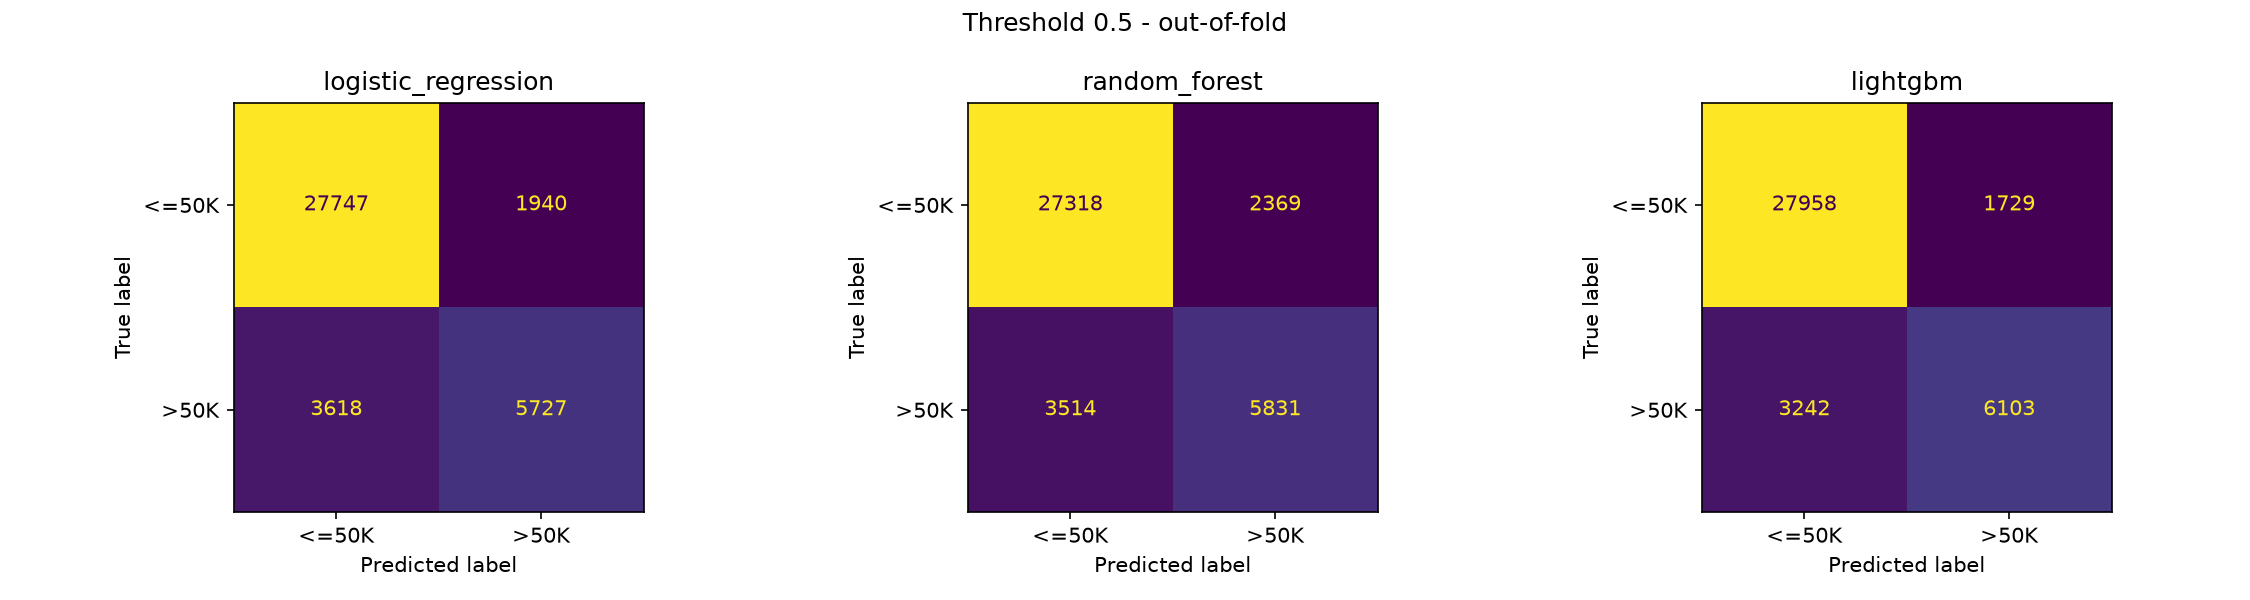
\includegraphics[width=0.9\textwidth]{baseline_confusion_default.png}\\[4pt]
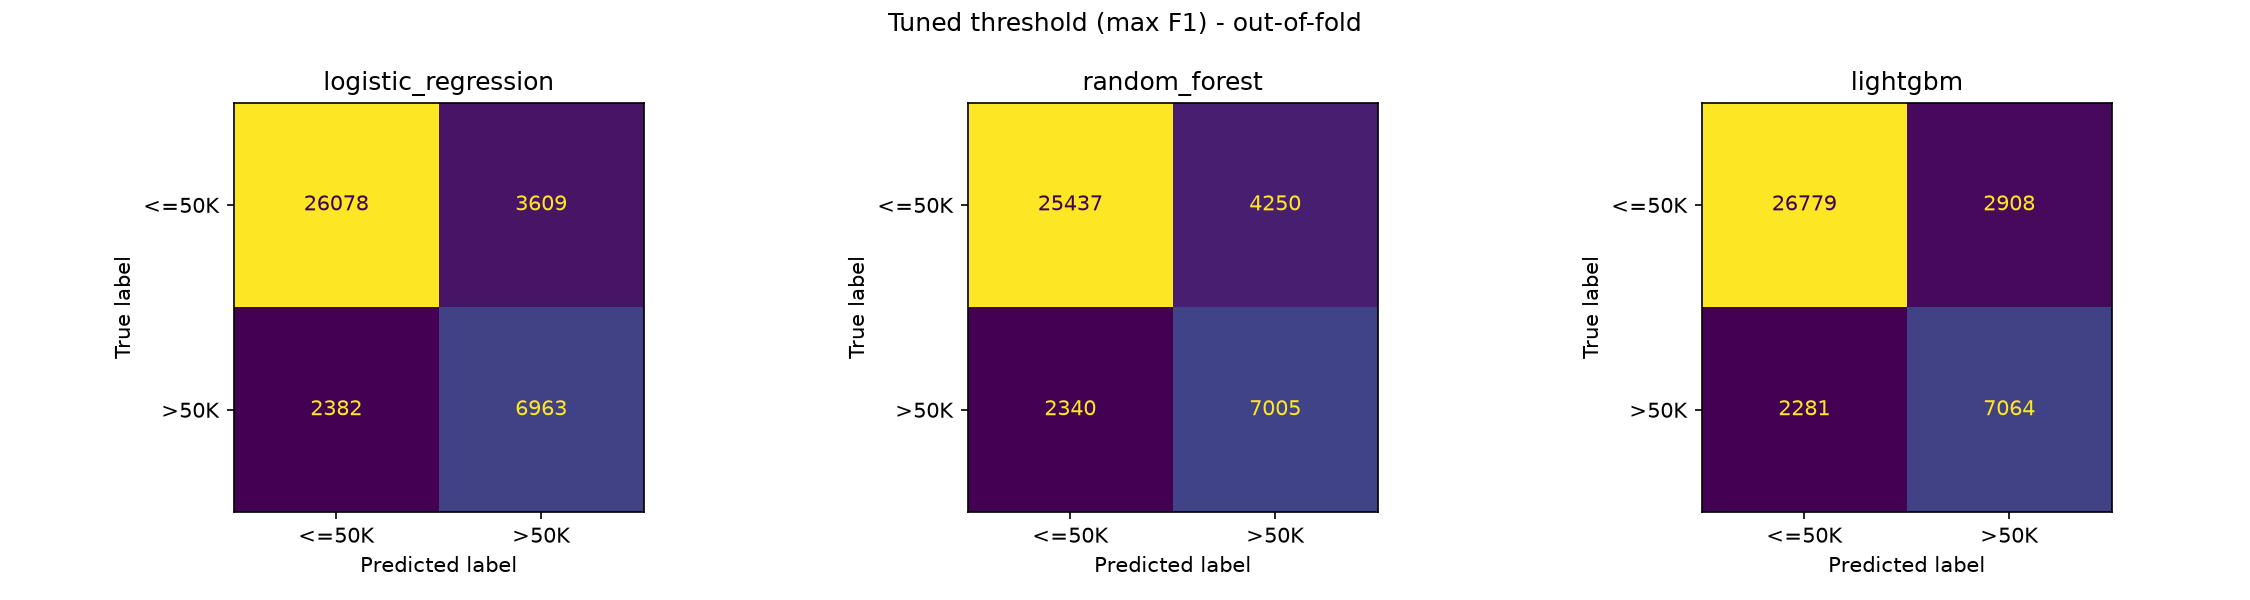
\includegraphics[width=0.9\textwidth]{baseline_confusion_tuned.png}
\caption{Out-of-fold confusion matrices of the untuned models, at the threshold
0.5 (top) and at the threshold that maximizes F1 (bottom).}
\label{fig:confusion-baseline}
\end{figure}

\paragraph{Chosen remedy.} We keep both levers, each in its place. The class
weight becomes a hyperparameter that Optuna may use or not
(Section~\ref{sec:tuning}): \code{class\_weight} $\in$ \{None, balanced\} for
the logistic regression and the random forest, and \code{scale\_pos\_weight}
$\in [1, 3.18]$ for LightGBM. Then the decision threshold is chosen on the
out-of-fold probabilities of each tuned model and frozen before the test set
is used. Section~\ref{sec:calibration} comes back to the price of class
weighting on the probabilities.

\section{Modelling progression}
\label{sec:models}

\todo{three models, same metrics, what each step bought (untuned and tuned)}

\section{A single Pipeline}
\label{sec:pipeline}

All the preprocessing and the model are wrapped in one scikit-learn
\code{Pipeline}, which takes a raw census row and returns $P(\pos)$:
(1) a stateless \code{FunctionTransformer} adds the three engineered features;
(2) a \code{ColumnTransformer} applies median imputation and
\code{StandardScaler} to the numerical columns, most-frequent imputation and
\code{OneHotEncoder(handle\_unknown="ignore")} to the categorical ones, and
drops \code{education} and \code{fnlwgt} (\code{remainder="drop"}); (3) the
classifier. One Pipeline brings four guarantees.
\begin{itemize}
  \item \textbf{No leakage during cross-validation.} A fresh, unfitted copy
  (\code{clone}) is fitted in each fold, so the medians, means, standard
  deviations and categories are learned on the four training folds only.
  Imputing or scaling the whole development set first would have let each
  validation fold influence its own preprocessing.
  \item \textbf{The same transformations everywhere.} The same object is
  cross-validated, refitted on the whole development set, evaluated on the
  test set and saved: no second implementation of the preprocessing can drift
  from the first one.
  \item \textbf{Tuning covers the whole chain.} Each Optuna trial builds and
  cross-validates a complete Pipeline (Section~\ref{sec:tuning}).
  \item \textbf{One file to deploy.} The fitted Pipeline is saved with
  \code{joblib}, together with its decision threshold, since both are needed
  to turn a raw row into a decision. It also returns the name of each encoded
  column (\code{get\_feature\_names\_out}), which the SHAP analysis uses.
\end{itemize}

\section{Hyperparameter tuning}
\label{sec:tuning}

\paragraph{Protocol.} We tuned each model with Optuna and its TPE sampler
(seed 42, so a re-run proposes the same trials). One trial is one
configuration and one cross-validated score:
\begin{enumerate}
  \item Optuna proposes a set of hyperparameters;
  \item we build the complete Pipeline with them (features, preprocessing,
  model);
  \item we score it with the same 5-fold stratified cross-validation on the
  development set;
  \item Optuna receives the mean AP over the 5 folds, and uses all the past
  trials to choose the next configuration.
\end{enumerate}
The budget is 25 trials for the logistic regression, 20 for the random forest
(the slowest to fit) and 50 for LightGBM, which has the largest search space.
A grid search would not fit this budget: with only three values for each of
LightGBM's eight hyperparameters, it would need $3^8 = 6{,}561$
configurations, i.e.\ about 33{,}000 fits with 5-fold CV. A random search would
fit the budget, but it ignores the scores of past trials, whereas Optuna's TPE
sampler uses them to spend more trials in the promising regions of the space.
The search spaces are given in Table~\ref{tab:search-spaces} (appendix). They
include the class weighting (Section~\ref{sec:imbalance}), from no weight at
all up to the class ratio. We optimize AP because it judges the ranking of the
minority class without depending on a threshold, which is chosen afterwards.

\paragraph{Why the best CV score is optimistic.} The best of 20 to 50 trials is
selected on the same folds that score it, so part of its advantage is luck on
these particular folds. The best mean CV AP is therefore an optimistic estimate
of performance, and we do not report it as our final result: the honest
estimate comes from the test set, which played no role in tuning
(Section~\ref{sec:test}). Nested cross-validation would remove this bias
without a test set, but it would multiply the cost of tuning by five; with
48{,}790 rows, a held-out test set was the cheaper way to get an unbiased
estimate.

\paragraph{Final training.} For each model, \code{train.py} then
(1) computes the out-of-fold probabilities of the tuned Pipeline on the same 5
folds, (2) chooses the threshold that maximizes F1 on them and freezes it,
(3) refits the Pipeline on the whole development set, and (4) saves the fitted
Pipeline with its threshold. The final model is the one with the best
out-of-fold AP.

\paragraph{Results.} Table~\ref{tab:best-params} gives the best configuration
of each model and its mean CV AP.

\begin{table}[H]
\centering
\caption{Best hyperparameters found by Optuna and best mean CV AP.}
\label{tab:best-params}
\small
\begin{tabular}{lp{8.5cm}r}
\toprule
Model & Best hyperparameters & CV AP \\
\midrule
Logistic regression & $C = 1.89$, \code{l1\_ratio} $= 0.77$ (Elastic Net, mostly
Lasso), no class weight & 0.784 \\
Random forest & 200 trees, \code{max\_depth} $= 14$, \code{min\_samples\_leaf}
$= 3$, \code{max\_features} $= 0.60$, \code{class\_weight="balanced"} & 0.815 \\
LightGBM & 350 trees, learning rate $0.048$, 26 leaves,
\code{min\_child\_samples} $= 11$, \code{subsample} $= 0.81$,
\code{colsample\_bytree} $= 0.57$, $\lambda = 0.015$,
\code{scale\_pos\_weight} $= 1.80$ & 0.833 \\
\bottomrule
\end{tabular}
\end{table}

Three observations:
\begin{itemize}
  \item \textbf{Edges of the ranges.} Only one value landed at the edge of its
  range: \code{max\_features} $= 0.60$ for the random forest, the upper bound.
  Letting each split see more features might still help the forest a little;
  we did not extend the range because the forest stays well behind LightGBM.
  All the other values are inside their ranges.
  \item \textbf{Class weighting.} Optuna made three different choices: no
  weight for the logistic regression, \code{"balanced"} for the random forest,
  and a moderate weight of 1.80 for LightGBM, about half of the class ratio
  (3.2). Since the threshold is tuned afterwards in every case, the weight is
  just one more hyperparameter, kept only when it improves AP.
  \item \textbf{A flat optimum for LightGBM.} Its best trial is trial 2: the 47
  following trials did not beat it (Figure~\ref{fig:lgbm-history}). Many
  configurations reach about the same AP, so more trials would not change the
  model much.
  \item \textbf{The learning rate.} Its range, 0.01 to 0.2 on a log scale,
  covers the usual values, and the trials show why the optimum is flat. Below
  0.02, even 1{,}000 trees are not enough to finish learning (mean AP 0.811
  over 2 trials). Above 0.1, each tree corrects too much at once (mean AP
  0.826 over 21 trials). Between 0.02 and 0.1, the 27 trials average 0.829
  and the ten best all lie within 0.002 AP, about the variation across folds.
  The selected $\eta = 0.048$ with 350 trees is therefore one good point of a
  plateau rather than a sharp optimum; the number of trees was chosen by
  cross-validation together with $\eta$, not by early stopping.
\end{itemize}

\begin{figure}[H]
\centering
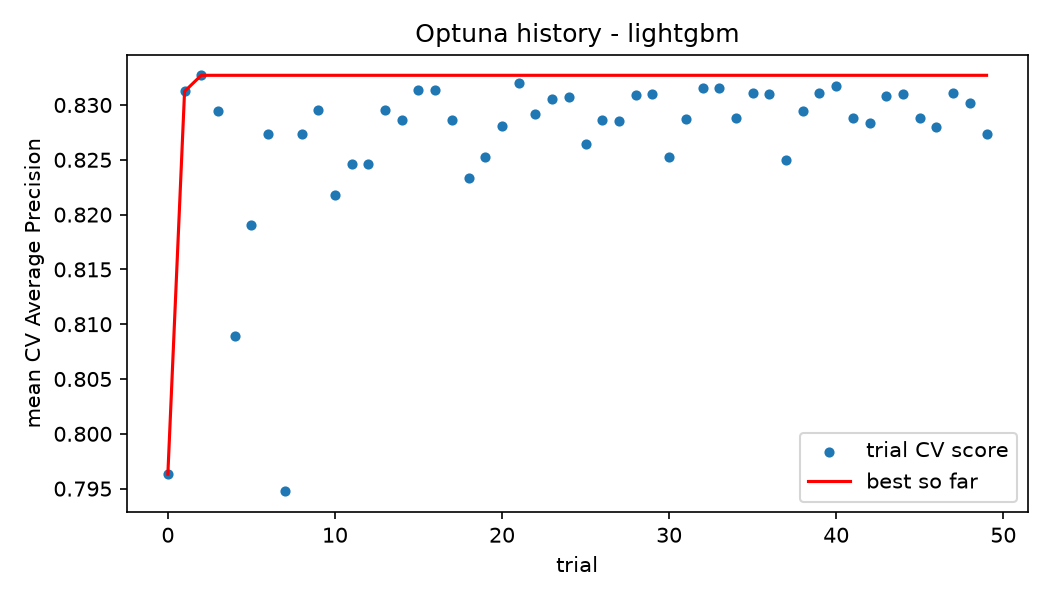
\includegraphics[width=0.65\textwidth]{lightgbm_history.png}
\caption{Mean CV AP of each Optuna trial for LightGBM.}
\label{fig:lgbm-history}
\end{figure}

\subsection{What the penalty does to the logistic regression}
\label{sec:regularization}

To see what the tuned penalty does, we look at the coefficients of the
final logistic regression and at the regularization path: train and validation
AP (5-fold CV, development set) for $C$ from $10^{-4}$ to $100$, with
\code{l1\_ratio} kept at its tuned value of 0.77
(Figure~\ref{fig:regularization-path}, script \code{src/regularization.py}).

\begin{itemize}
  \item \textbf{Sparsity.} The L1 part of the penalty sets 9 of the 91
  coefficients exactly to zero: seven \code{native-country} categories, mostly
  rare ones (Ecuador, Honduras, Holand-Netherlands, \dots), \code{workclass} =
  Never-worked, and \code{relationship} = Not-in-family, which carries
  little extra information once marital status and the other relationship
  categories are known. A Ridge penalty would only have shrunk them.
  \item \textbf{Strong penalty = underfitting.} At $C = 10^{-4}$ every
  coefficient is zero and the model predicts the base rate for everyone (AP
  0.24, the share of >50K). As $C$ grows, the model keeps more coefficients
  (7 at $C = 10^{-3}$, 39 at $C = 0.1$) and AP rises quickly.
  \item \textbf{Weak penalty does not overfit here.} Above $C \approx 0.1$
  the validation AP is flat (0.782 to 0.784), and the gap between train and
  validation AP stays below 0.004 even at $C = 100$. With about 39{,}000 rows
  for 91 coefficients, the model has too few parameters to memorize the
  training folds. This explains why tuning did not improve the logistic
  regression (Section~\ref{sec:models}): the tuned $C = 1.89$ lies in a
  flat region where the strength of the penalty barely matters.
  \item \textbf{A simpler model at almost no cost.} With $C = 0.1$, 39
  coefficients reach AP 0.782 against 0.784 with all 91. If a short, readable
  model mattered more than the last 0.002 AP, this stronger penalty would be
  the better choice.
\end{itemize}

\begin{figure}[H]
\centering
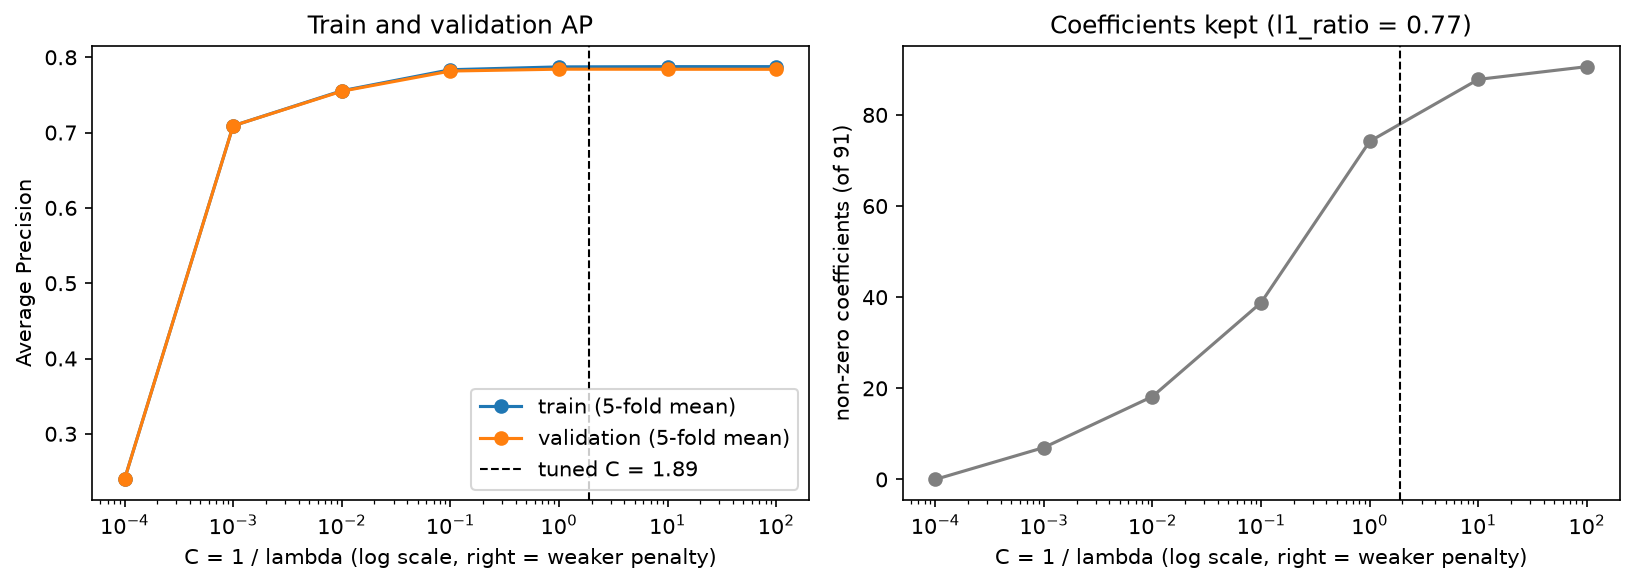
\includegraphics[width=\textwidth]{regularization_path.png}
\caption{Regularization path of the logistic regression (\code{l1\_ratio} =
0.77). Left: mean train and validation AP over the 5 folds. Right: mean number
of non-zero coefficients. Dashed line: the tuned $C$.}
\label{fig:regularization-path}
\end{figure}

\section{Experiment tracking}
\label{sec:tracking}

Every tuning trial and every final training is logged with MLflow, in a local
database (\code{mlflow.db}, with the files in \code{mlruns/}), under a single
experiment, \code{adult-income}:
\begin{itemize}
  \item \textbf{one parent run per tuning study} (e.g.\ ``lightgbm - tuning''):
  the best hyperparameters, the best mean CV AP, and the tuning files as
  artifacts (best parameters, table of all trials, optimisation history);
  \item \textbf{one child run per Optuna trial}: its hyperparameters, the AP of
  each of the 5 folds, their mean and standard deviation. Logging the five
  folds, not only the mean, shows how much a score depends on the split;
  \item \textbf{one run per final training}: the tuned hyperparameters, the
  out-of-fold metrics, the chosen threshold and the saved model as an artifact.
\end{itemize}
In total, the 95 tuning trials (25 + 20 + 50), the 3 tuning studies and the 3
final trainings are logged (Figure~\ref{fig:mlflow}, appendix). Since the
sampler and the folds are seeded, re-running the tuning with tracking switched
on proposes the same trials: the best hyperparameters, the frozen thresholds
and the out-of-fold scores of the three models were identical after the re-run.

\section{Explainability with SHAP}
\label{sec:shap}

\paragraph{Method.} SHAP splits one prediction into a reference value plus one
contribution per feature: $f(x) = \phi_0 + \sum_j \phi_j(x)$, where $\phi_0$ is
the base value. For LightGBM, \code{TreeExplainer} computes these values
exactly, in log-odds of \pos: a positive value pushes the prediction towards
\pos. We explain the final model on 1{,}000 people drawn from the development
set; the test set stays untouched. One-hot encoding splits each categorical
feature into several columns, and SHAP values are additive, so we sum the
values of the columns of each original feature (e.g.\ all the
\code{relationship} columns) to get one contribution per feature. As a check,
for every explained person, the base value plus the sum of the contributions
gives back the raw score, and its sigmoid gives back the predicted probability.

\paragraph{Global importance.} The global importance of a feature is its mean
absolute SHAP value over the 1{,}000 people: how much it moves the
predictions on average, whatever the direction. The beeswarm plot adds the
direction (Figure~\ref{fig:shap-global}). Marital status comes first by far
(mean $|\text{SHAP}|$ of 0.93 in log-odds), followed by age (0.58), capital
gains (0.53), relationship (0.41) and our interaction
\code{education\_x\_hours} (0.39); occupation (0.31) and \code{education-num}
(0.30) come next. Sex is 9th (0.18) and race 14th (0.06) out of 15.

The beeswarm, drawn per encoded column before the sum, shows the direction of
each effect. Being married to a civilian spouse pushes the score up by about
$+0.8$, and not being married pulls it down by about as much. Young ages pull it
down strongly (to about $-2.5$), while middle and older ages push it up. Most
people have no capital gain, which pulls the score down slightly, but a large
gain pushes it up by $+4$ to $+7$: the largest single effects of the model.
Higher education and more \code{education\_x\_hours} push the score up.

\begin{figure}[H]
\centering
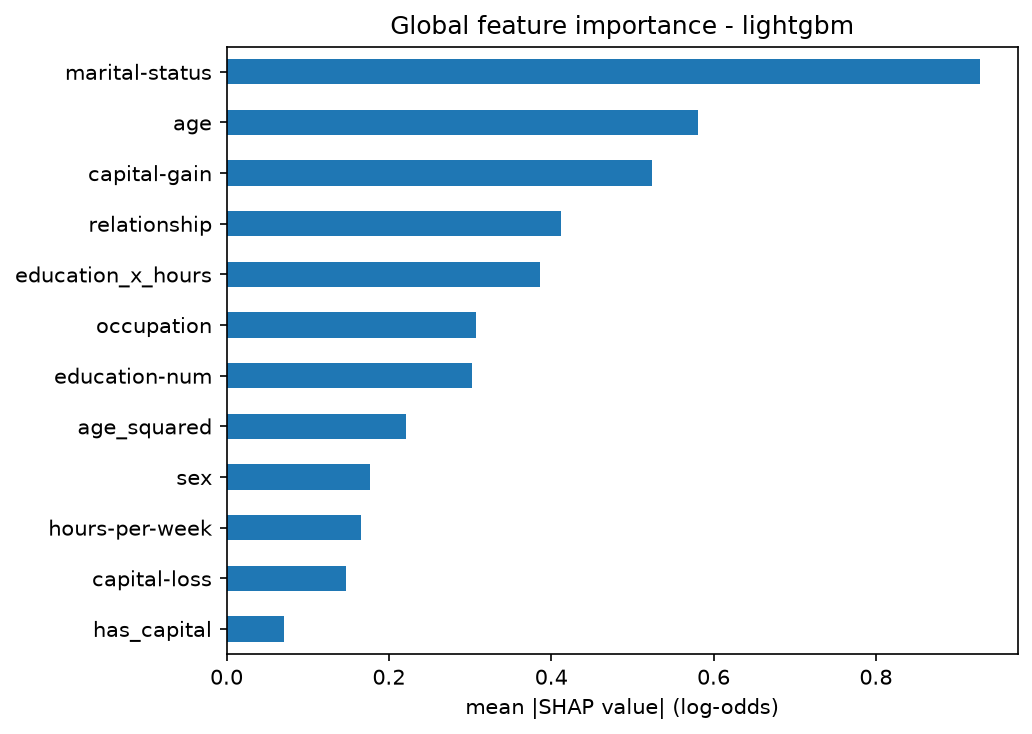
\includegraphics[width=0.48\textwidth]{shap_global_importance.png}\hfill
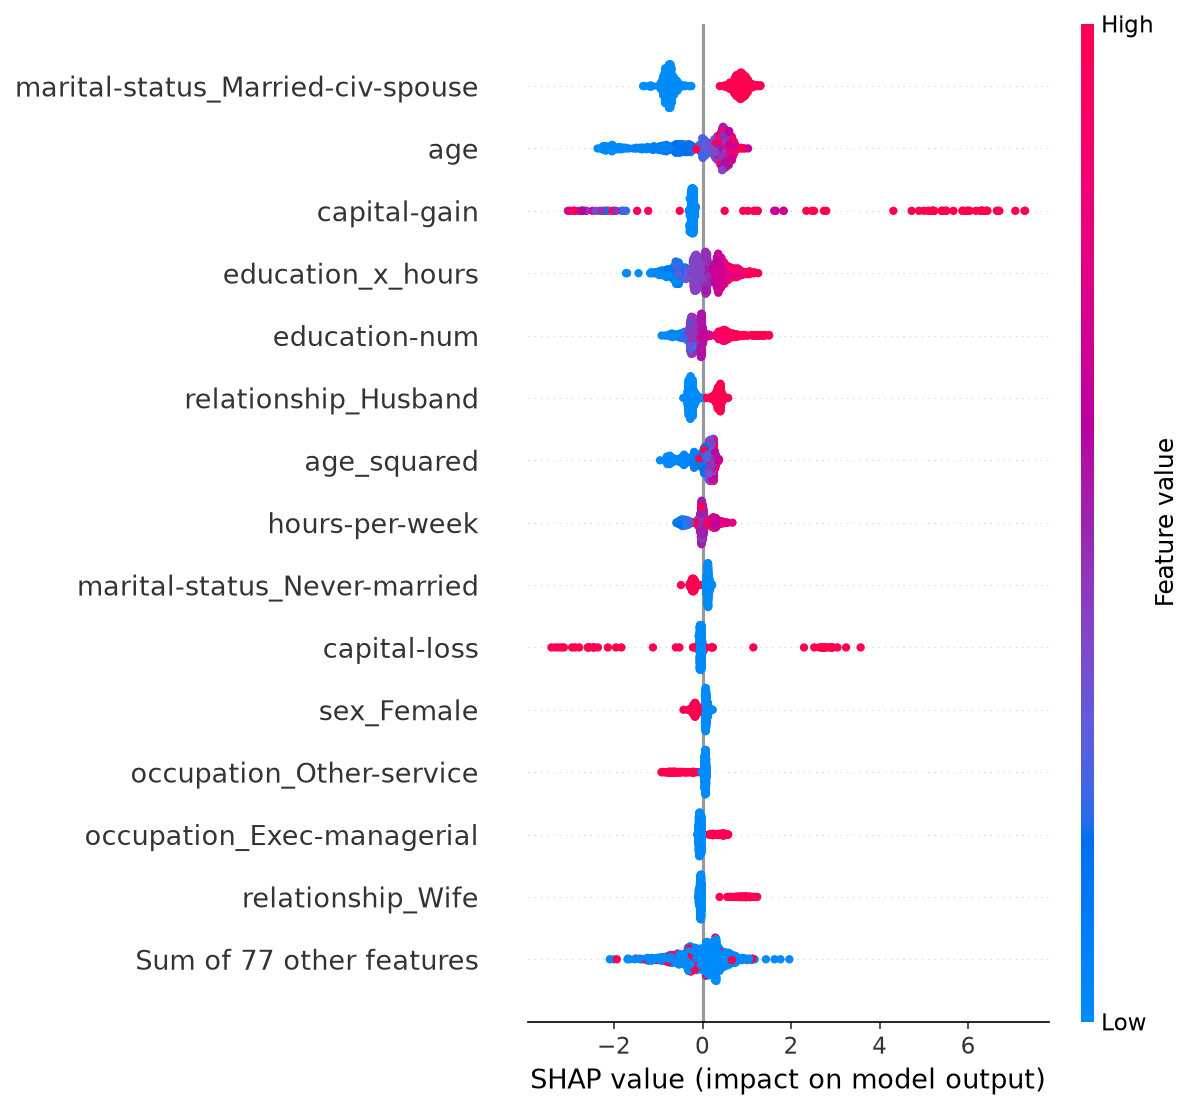
\includegraphics[width=0.48\textwidth]{shap_beeswarm.png}
\caption{Global SHAP importance per original feature (left) and beeswarm plot
per encoded column (right) of the final model, on 1{,}000 people of the
development set.}
\label{fig:shap-global}
\end{figure}

\paragraph{Local explanations.} We explain three people: the most confident
\pos{} prediction, the most confident \negc{} prediction, and the person
closest to the decision threshold (Figure~\ref{fig:shap-local}). All three
start from the base value $\phi_0 = -1.93$ (a probability of 0.13).
\begin{itemize}
  \item \textbf{Most confident \pos{}} ($P = 0.999$, truly \pos). A capital
  gain of \$15{,}024 adds $+5.67$ on its own, more than half of the total
  push of $+9.26$. Being married ($+0.74$), 16 years of education ($+0.61$),
  their product with 50 hours a week ($+0.50$) and an executive job ($+0.39$)
  add the rest.
  \item \textbf{Most confident \negc{}} ($P < 0.001$, truly \negc). Age 18 is
  the main reason: $-2.17$ for \code{age} and $-0.79$ for
  \code{age\_squared}. Little education times few hours ($-1.18$), never
  married ($-0.90$) and a farming job ($-0.50$) push in the same direction.
  \item \textbf{Closest to the threshold} ($P = 0.539$, just below the
  threshold of 0.54, so predicted \negc; truly \negc). A married man of 35
  with a high \code{education\_x\_hours}: being married ($+0.88$), the
  interaction ($+0.63$) and being a husband ($+0.36$) push up, but the absence
  of capital gains ($-0.21$) keeps him just under the threshold.
\end{itemize}

\begin{figure}[H]
\centering
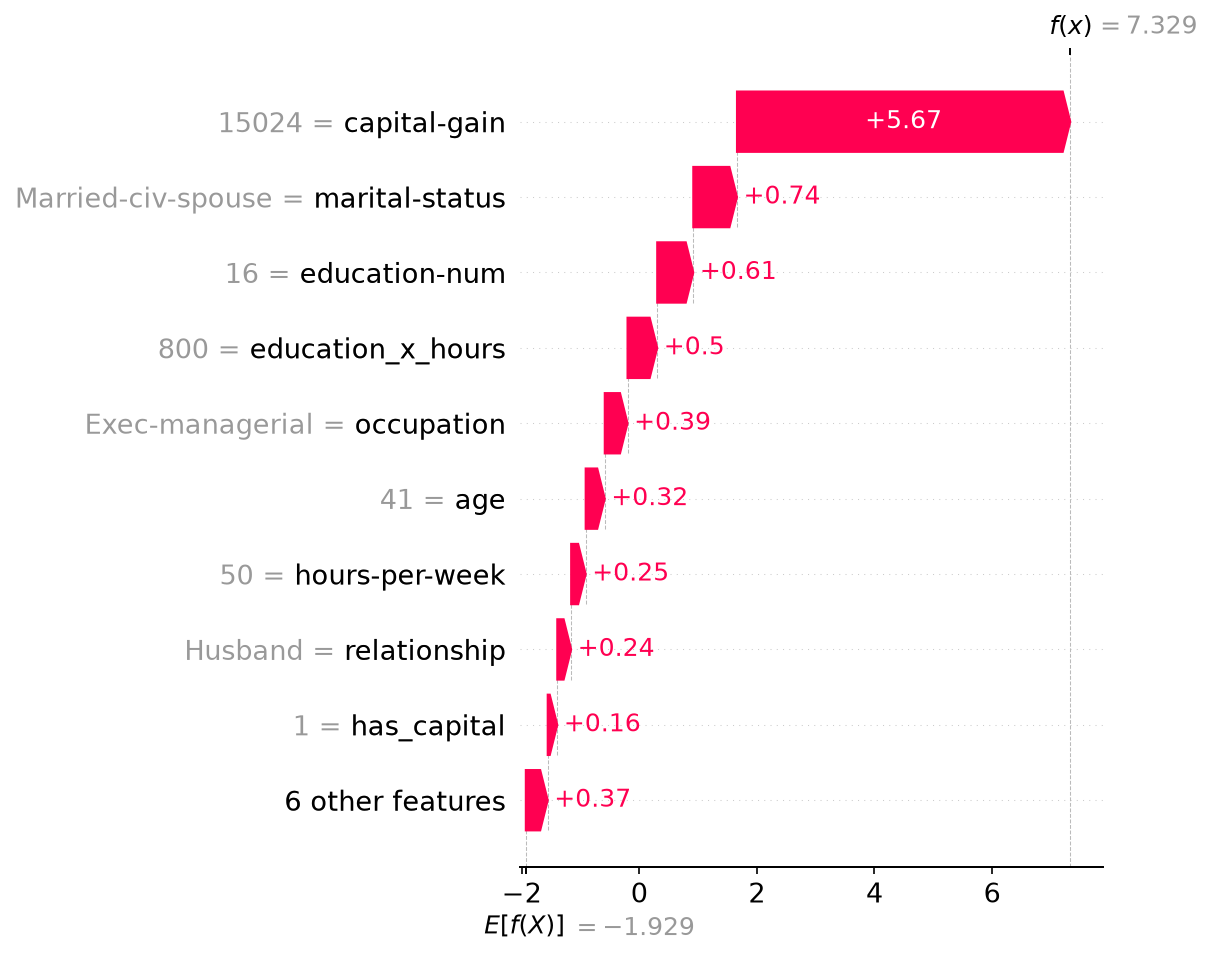
\includegraphics[width=0.48\textwidth]{shap_local_most_likely_above_50k.png}\hfill
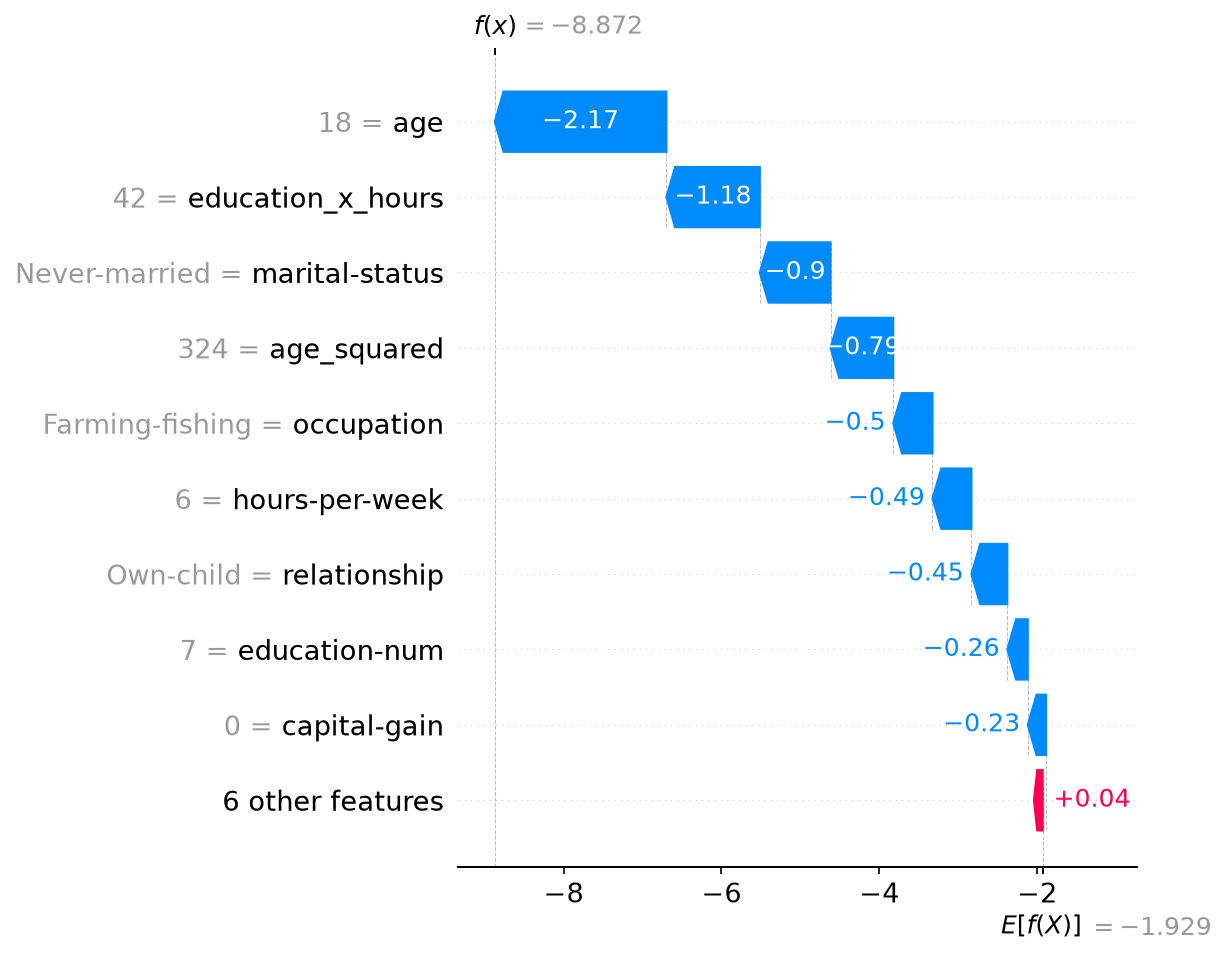
\includegraphics[width=0.48\textwidth]{shap_local_least_likely_above_50k.png}\\[4pt]
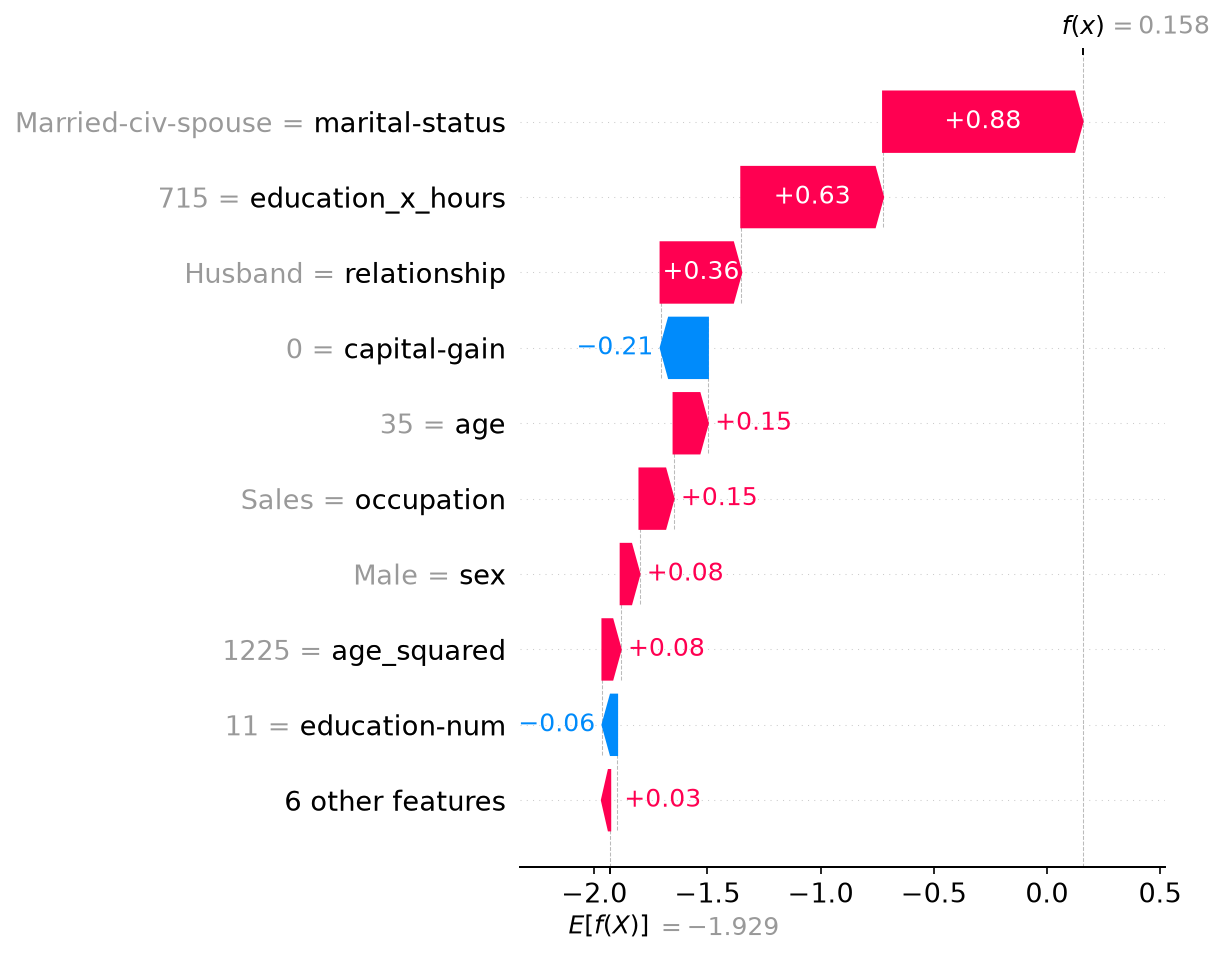
\includegraphics[width=0.48\textwidth]{shap_local_borderline.png}
\caption{Waterfall plots of the most confident \pos{} (top left), the most
confident \negc{} (top right) and the person closest to the threshold
(bottom): from the base value, each feature pushes the score up (red) or down
(blue) until the final prediction.}
\label{fig:shap-local}
\end{figure}

\paragraph{Do the important features make business sense?} Mostly yes. The
household variables come first (marital status and relationship together weigh
1.34): being married is a proxy for age, career stage and a stable household.
Capital gains are a direct sign of wealth, and age, education and occupation
describe a career. These are the drivers one would expect for income. Our
engineered features are used (Section~\ref{sec:features}):
\code{education\_x\_hours} is 5th, ahead of \code{education-num} itself, and
\code{age\_squared} is 8th; \code{has\_capital} is only 12th, because the trees
can split on \code{capital-gain} directly. Sex (9th) and race (14th) weigh
less, but not zero: being a woman lowers the score by about $0.3$ in log-odds
in the beeswarm, on top of what passes through \code{relationship}
(\code{Husband} / \code{Wife}). The model reproduces the income gap between
men and women in the 1994 census; with the fairness audit out of scope, we
flag it as a limitation rather than measure it. Two cautions apply to this
reading. SHAP explains what the model
does, not what causes a high income: being married does not raise anyone's
income in itself. And correlated features share the credit: \code{age} and
\code{age\_squared}, \code{marital-status} and \code{relationship}, or
\code{education-num} and \code{education\_x\_hours} must be read together.

\section{Calibration diagnostics}
\label{sec:calibration}

\todo{reliability curve, Brier score, ECE, over- or under-confident, trust for a downstream decision}

\section{Final evaluation on the untouched test set}
\label{sec:test}

\todo{one evaluation of the three tuned models with their frozen thresholds}

\section{Alternatives tested, limitations and conclusion}
\label{sec:discussion}

\subsection{An alternative we tested: a ``missing'' category}

The analysis left an open question (Section~\ref{sec:eda}): are the missing job
values random? On the development set, the 2{,}233 people with a missing
\code{workclass} all have a missing \code{occupation} too (2{,}241 missing
occupations in total: the other 8 people never worked), and only 9.4\% of the
people with a missing occupation earn \pos, against 23.9\% overall: they are
mostly people without a job. The most-frequent imputation hides this, since it
gives them the most common job (\code{Private}, \code{Prof-specialty}).
Imputing a separate ``missing'' category keeps the information. On the untuned
models (Table~\ref{tab:missing}, appendix), it gains 0.003 AP for the logistic
regression and 0.001 for LightGBM, with no change in F1 for LightGBM: of the
order of the variation of AP across folds. Adopting it would have meant
re-running the whole tuning for no measurable gain, so we kept the
most-frequent imputation. A separate category remains the more principled
choice for a model in production, because it does not invent a job for people
who have none.

\subsection{Overfitting: what we checked and what we did not}
\label{sec:overfitting}

\begin{itemize}
  \item \textbf{Overfitting the validation folds: checked.} The 95 Optuna
  trials and the thresholds were all chosen on the same 5 folds, so the best
  CV scores are optimistic by construction. The untouched test set measures by
  how much: every model loses about 0.01 AP (logistic regression 0.784 to
  0.773, random forest 0.814 to 0.805, LightGBM 0.832 to 0.821), and the
  ranking does not change. This is the drop expected from selection.
  \item \textbf{Memorizing the training rows: checked for the logistic
  regression only.} Its train--validation gap stays below 0.004 even with
  almost no penalty (Section~\ref{sec:regularization}). For the two tree
  models we never computed a training score. The evidence is indirect: the
  untuned random forest, whose leaves are pure, is the worst model, and
  limiting its depth and leaf size raised its CV AP by 0.064, which is what
  reducing overfitting looks like; LightGBM's 350 trees were chosen by CV
  rather than by early stopping.
\end{itemize}
For tree ensembles, a training score above the validation score is normal:
what matters is that the validation and test scores hold, and they do. A table
of train, validation and test AP for the three models, and a LightGBM learning
curve, would measure the size of the gap.

\subsection{Limitations}

\begin{itemize}
  \item \textbf{Old data.} The census dates from 1994; incomes, jobs and the
  meaning of \$50K have changed, so the model would need retraining on recent
  data.
  \item \textbf{Possible leakage.} \code{capital-gain} and \code{capital-loss}
  are declared for the same tax year as the income (Section~\ref{sec:eda}).
  \item \textbf{F1 stands in for business costs.} With real costs for each
  type of error, the threshold should minimize the expected cost instead.
  \item \textbf{Threshold chosen on fold models.} It comes from the
  out-of-fold probabilities of five models trained on 80\% of the development
  set, and is applied to a model refitted on all of it; their scores are close
  but not identical.
  \item \textbf{Probabilities not calibrated} as-is
  (Section~\ref{sec:calibration}), and overfitting of the tree models not
  measured directly (Section~\ref{sec:overfitting}).
  \item \textbf{No fairness audit.} The model uses \code{sex} and \code{race}
  as inputs, and the share of \pos{} is 30\% for men against 11\% for women.
  The audit was removed from the scope, so we did not check whether errors are
  spread equally across groups; this would be needed before any real use.
\end{itemize}

\subsection{Conclusion}

Our final model is a tuned LightGBM inside a single scikit-learn Pipeline. On
the untouched test set it reaches an AP of 0.821 and an F1 of 0.722 at its
frozen threshold of 0.54, within 0.01 of its cross-validation scores. What
mattered most was the choice of model (LightGBM is about 0.05 AP ahead of the
logistic regression), then the decision threshold, then the engineered
features. Its decisions are reliable, but its raw probabilities are
over-estimated because of the class weight, so they should be recalibrated
before being read as true chances (Section~\ref{sec:calibration}).

\section*{Contribution statement}
\addcontentsline{toc}{section}{Contribution statement}

\begin{table}[H]
\centering
\begin{tabular}{lll}
\toprule
Requirement or stage & Main author & Reviewed by \\
\midrule
Repository, data loading and split (1) & Eduardo & Jules \\
EDA and problem framing (1) & Eduardo & Jules \\
Feature engineering (2) & Eduardo & Jules \\
Class imbalance (3) & Eduardo & Jules \\
Modelling progression (4) & Eduardo & Jules \\
Pipeline (5) & Eduardo & Jules \\
Optuna tuning, final training, test evaluation (6) & Eduardo & Jules \\
Experiment tracking with MLflow (7) & Louis & Eduardo, Jules \\
SHAP explainability (8) & Louis & Jules \\
Calibration diagnostics (9) & Louis & Jules \\
Code review and fixes, alternatives tested (Section~\ref{sec:discussion}) & Jules & Eduardo, Louis \\
Report & All three & All three \\
\bottomrule
\end{tabular}
\end{table}

\section*{Use of AI coding assistants}
\addcontentsline{toc}{section}{Use of AI coding assistants}

We used Claude (Anthropic), through the Claude Code assistant, to draft parts
of the code, to review it and suggest fixes, and to help structure and draft
this report. Eduardo's and Jules's commits written with its help carry a
``Co-Authored-By: Claude'' line in the Git history; Louis's commits for
steps 7 to 9 were also written with its help but do not carry this line.
Every methodological choice was discussed by the team, every number in this
report comes from running our own scripts, and each member can explain the
code.


\clearpage
\appendix
\section{Additional material}
\label{sec:appendix}

\subsection{Optuna search spaces}

\begin{table}[H]
\centering
\caption{Search spaces of the three models. ``log'': sampled on a log scale.
$r = N_{\text{neg}}/N_{\text{pos}} \approx 3.18$ on the development set.}
\label{tab:search-spaces}
\small
\begin{tabular}{lll}
\toprule
Model (trials) & Hyperparameter & Range \\
\midrule
Logistic regression (25) & \code{C} & $[10^{-3}, 10]$, log \\
                         & \code{l1\_ratio} & $[0, 1]$ \\
                         & \code{class\_weight} & None or balanced \\
\midrule
Random forest (20) & \code{n\_estimators} & 100 to 300, step 50 \\
                   & \code{max\_depth} & 4 to 24 \\
                   & \code{min\_samples\_leaf} & 1 to 50, log \\
                   & \code{max\_features} & $[0.1, 0.6]$ (share of the columns) \\
                   & \code{class\_weight} & None or balanced \\
\midrule
LightGBM (50) & \code{n\_estimators} & 100 to 1000, step 50 \\
              & \code{learning\_rate} & $[0.01, 0.2]$, log \\
              & \code{num\_leaves} & 8 to 128, log \\
              & \code{min\_child\_samples} & 5 to 100, log \\
              & \code{subsample} & $[0.5, 1]$, applied at every iteration \\
              & \code{colsample\_bytree} & $[0.5, 1]$ \\
              & \code{reg\_lambda} & $[10^{-3}, 10]$, log \\
              & \code{scale\_pos\_weight} & $[1, r]$ \\
\bottomrule
\end{tabular}
\end{table}

\subsection{Exploratory figures}

\begin{figure}[H]
\centering
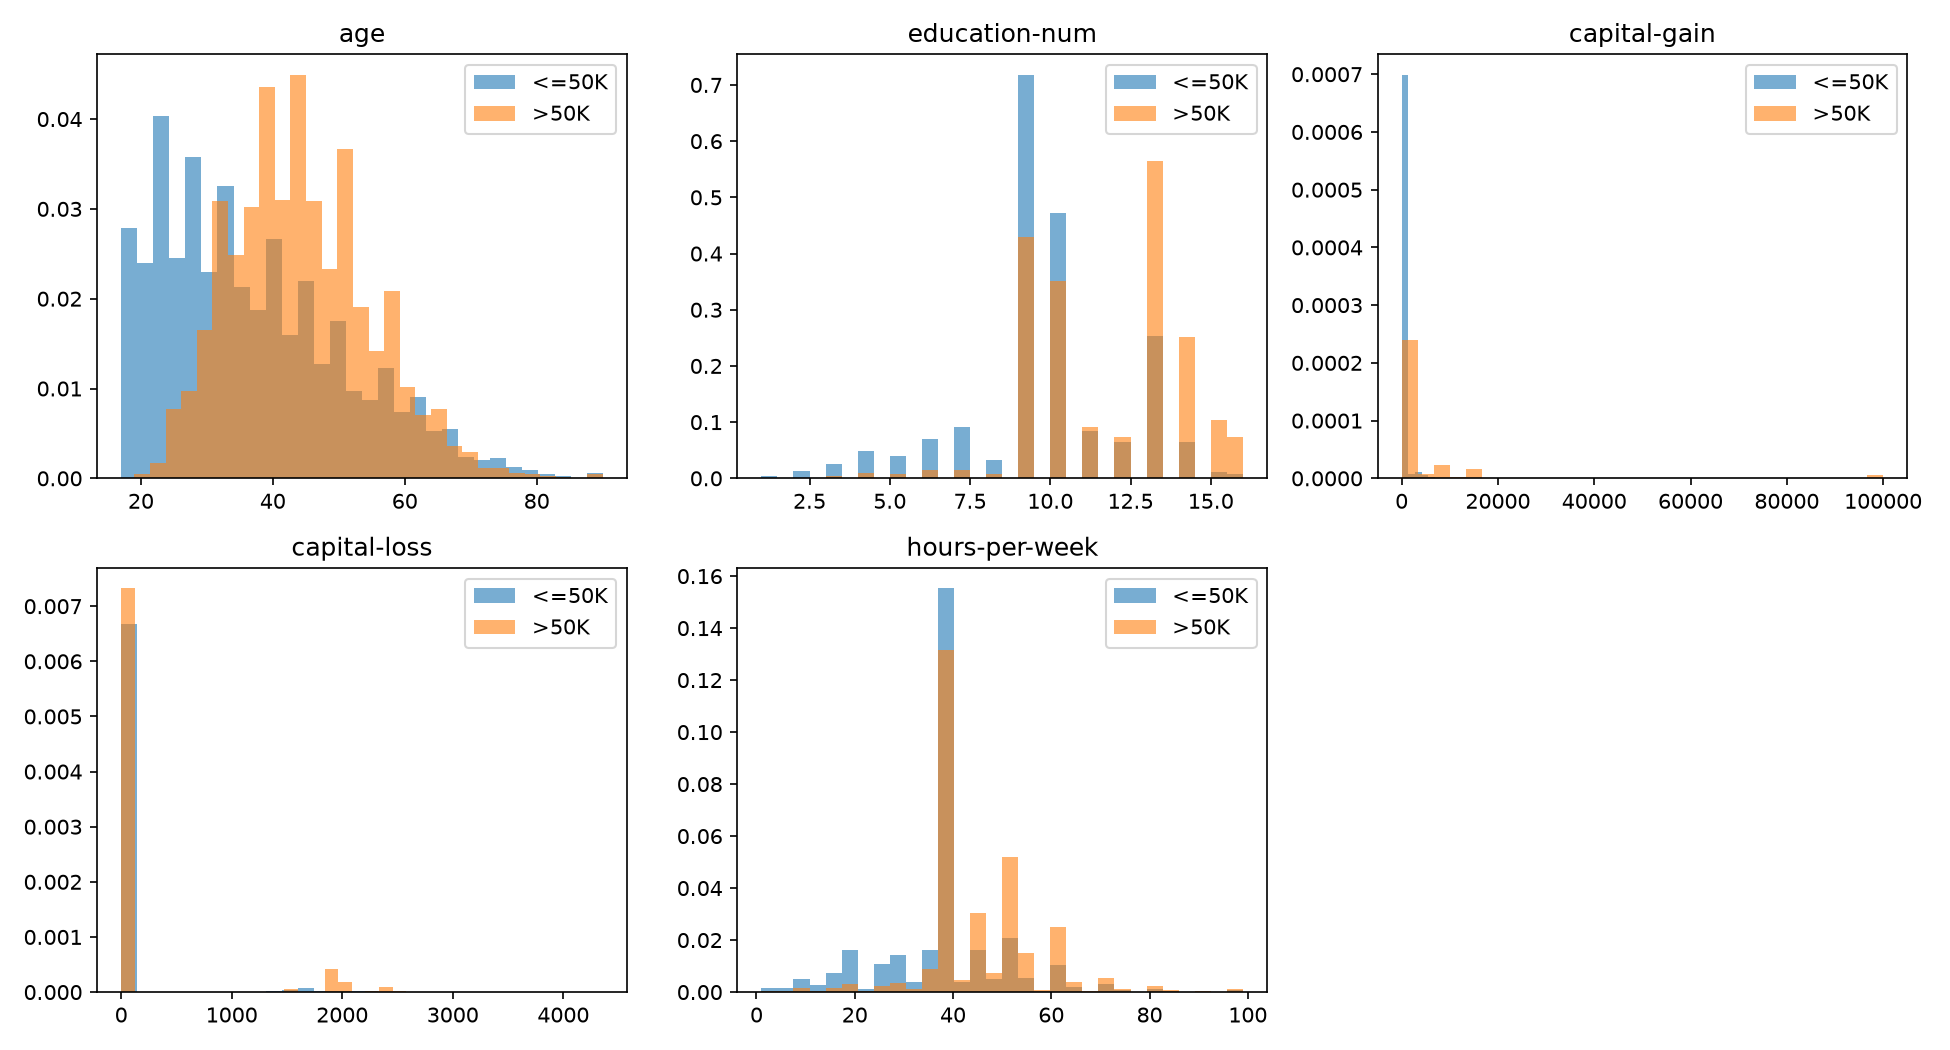
\includegraphics[width=0.95\textwidth]{eda_numeric_by_class.png}
\caption{Distribution of each numerical feature by class (development set,
densities).}
\label{fig:eda-numeric}
\end{figure}

\begin{figure}[H]
\centering
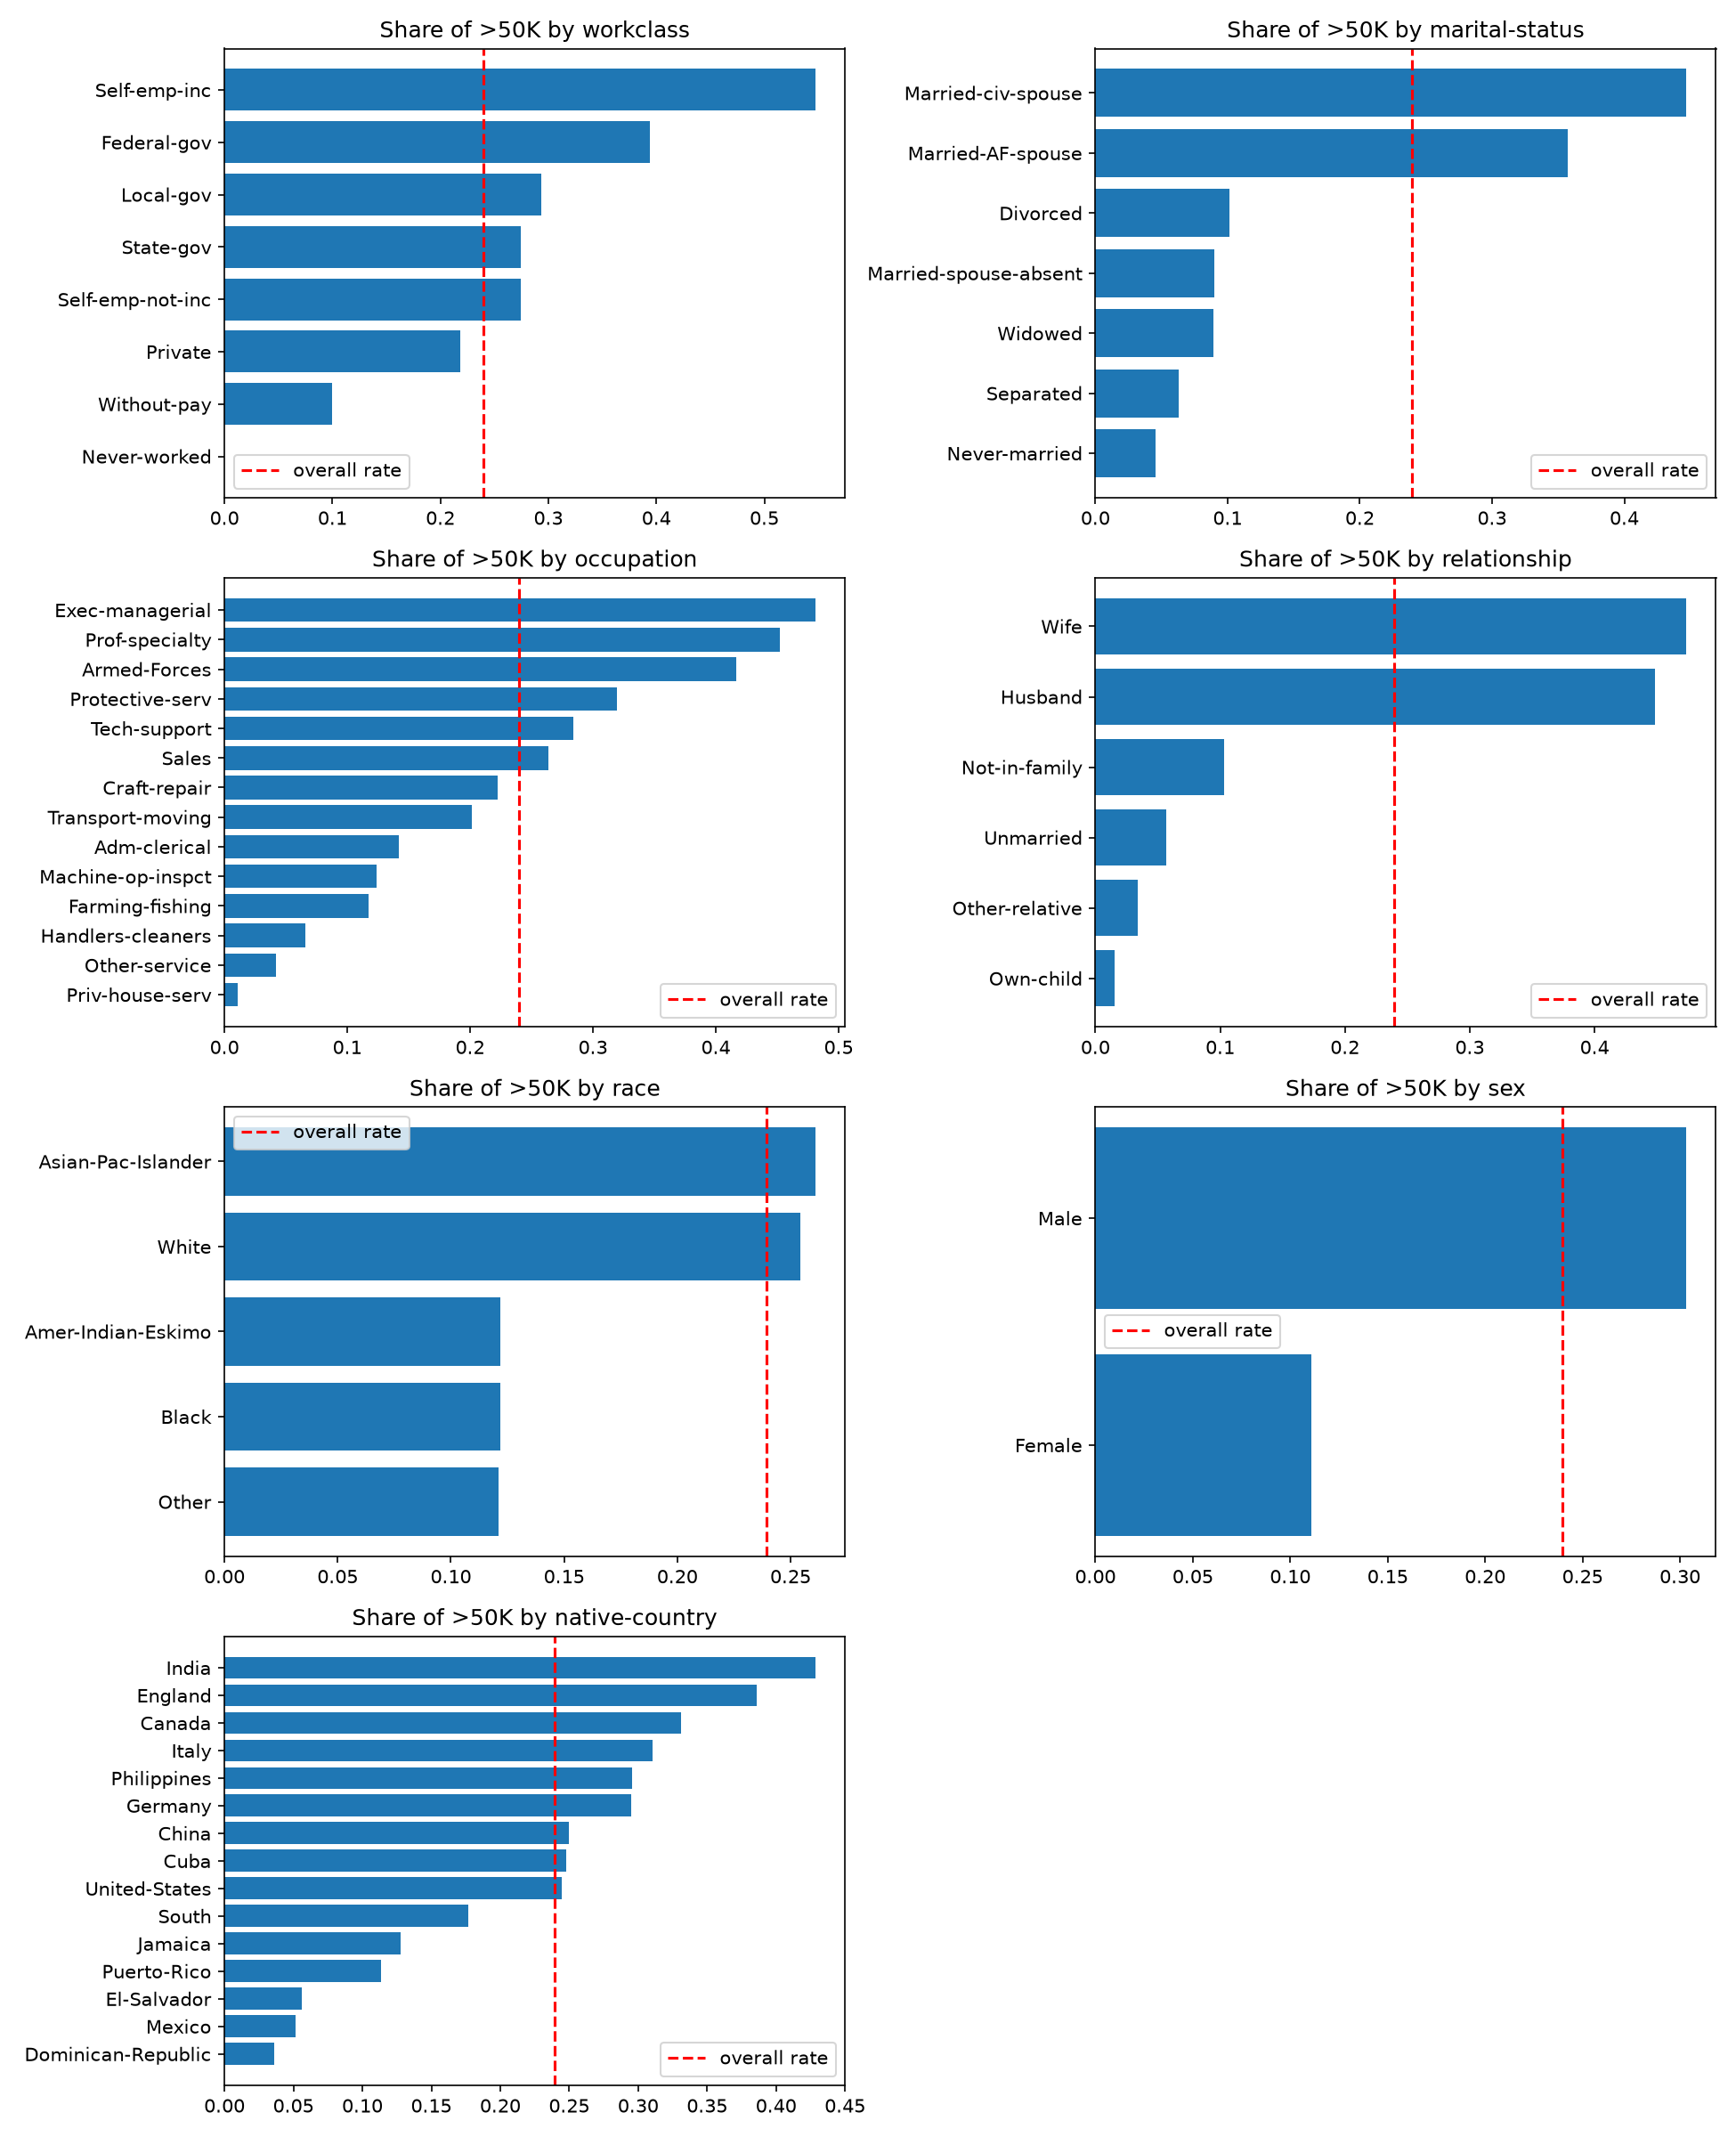
\includegraphics[width=0.85\textwidth]{eda_categorical_rates.png}
\caption{Share of \pos{} per category of each categorical feature (development
set). The dashed line is the overall share. For \code{native-country}, only the
15 most frequent countries are shown.}
\label{fig:eda-categorical}
\end{figure}


\end{document}
